% Created 2020-06-08 Mon 20:35
% Intended LaTeX compiler: pdflatex
\documentclass[11pt]{article}
\usepackage[utf8]{inputenc}
\usepackage[T1]{fontenc}
\usepackage{graphicx}
\usepackage{grffile}
\usepackage{longtable}
\usepackage{wrapfig}
\usepackage{rotating}
\usepackage[normalem]{ulem}
\usepackage{amsmath}
\usepackage{textcomp}
\usepackage{amssymb}
\usepackage{capt-of}
\usepackage{pdfpages}
\usepackage{ifthen}
\usepackage{hyperref}
\usepackage{caption}
\usepackage{minted}
\usepackage{minted}
\usepackage{amsmath}
\usepackage{pdftexcmds}
\usepackage{svg}
\usepackage{titling}
\renewcommand\maketitlehooka{\null\mbox{}\vfill}
\renewcommand\maketitlehookd{\vfill\null}

\newenvironment{code}{\captionsetup{type=listing}}{}
\usepackage[pdftex,letterpaper,margin=1.0in]{geometry}
\author{Michael Lynch}
\date{\today}
\title{C++ AutoGarbage\\\medskip
\large An automatic mark and sweep garbage collector for the C++ Programming Language}
\hypersetup{
 pdfauthor={Michael Lynch},
 pdftitle={C++ AutoGarbage},
 pdfkeywords={},
 pdfsubject={},
 pdfcreator={Emacs 25.2.2 (Org mode 9.2.1)}, 
 pdflang={English}}
\begin{document}

\begin{titlingpage}
\maketitle
\end{titlingpage}

\newpage
\vspace*{0.15\textheight}
\emph{Abstract.} C++ has become one of the most popular languages in the world, partially through its capability for very deep control
over memory mangement.
This project takes advantage of C++ power over direct memory, to implement an automatic garbage collection system
similar to those found in more high level languages such as Java or C\#.

\newpage
\tableofcontents
\newpage

\section{Usage}
\label{sec:orgad3520d}
The use of several classes and macros are required in order for the user to take advantage of the AutoGarbage memory management system.
To start AutoGarbage (AGC), the heap needs to be initiated using:

\begin{minted}[]{c++}
gc::init_gc(4096, 25);
\end{minted}

\begin{itemize}
\item The first parameter provides the size that the heap should be initiated to in bytes.
\item The second parameter indicates how many times the allocater should attempt to allocate an object before giving up and
performing a garbage collection.
\end{itemize}

AGC will heap allocate any object which inherits from the \texttt{gc::object} class.
AGC expects \texttt{gc::object} classes to be formatted with garbage collectable 
fields (\texttt{gc::field}) first followed by the \texttt{END\_GC\_FIELD} macro,
before standard C++ members in the classes memory map.

\begin{code}
\begin{minted}[]{c++}
class A : gc::object
{
  // These are garbage collectable objects.
  gc::field<B> _b;
  gc::field<C> _c;

  // This notifies that there are no more garbage collectable fields in the object.
  END_GC_FIELDS;

  //These are not pointer objects so get garbage collected along with the root object.
  int a;
  int b;
}
\end{minted}
\captionof{listing}{Example Object}
\end{code}


It is important to note that destructores for garbage collected objects are never called (objects just get overwritten once  emacs error logsthey are collected)
so it is inherantly unsafe to use any kind of standard C++ pointer (raw or smart) as a member on a gc::object unless you explicitly manage
creation and deletion of the objects yourself.
\subsubsection{Arrays:}
\label{sec:orgb60ee48}
AGC also supports garbage collectable reference arrays similar to ref arrays found in Java.

AGC supports runtime sized arrays throught the \texttt{gc::object} template class \texttt{gc::array<class T>}.

As an inheriter of \texttt{gc::object}, they can be placed in \texttt{gc::field} and \texttt{gc::static\_ptr} just like any other AGC object.

\texttt{gc::field} should be used to host AGC type members on classes.

\texttt{gc::static\_ptr} should be used in the scope of a program accessing AGC type members to ensure that it is not going to be garbage
collected before the program has finished using it.
\section{Technical Details}
\label{sec:orgf98330b}
\subsection{Marking}
\label{sec:orgbb9b100}
AGC relies on an obligation with how users layout their object classesas w work around for C++ lack of runtime reflection.

Garbage collectable fields are placed at the top of the class so that the marker knows where to start searching for fields.

C++ objects are formatted with the highest class in the inheritance tree placed first. This is done to make is easy to cast
one object to another without a dedicated runtime casting checker:


\begin{figure}[H]
%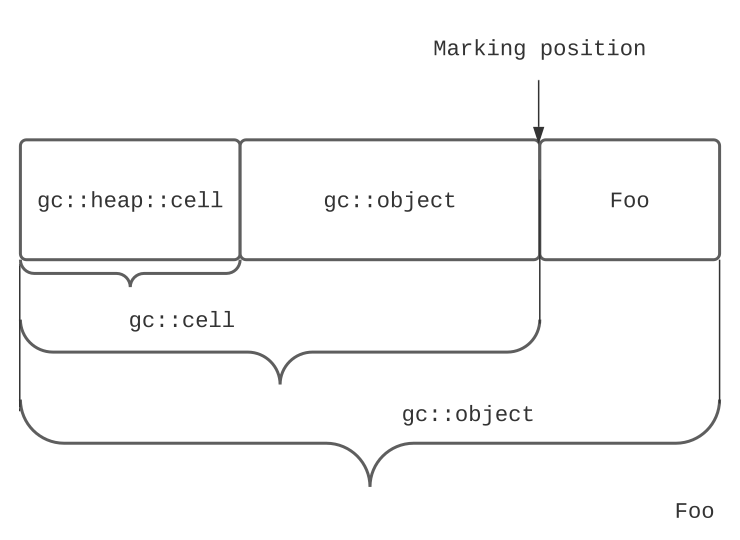
\includepdf[pages=1,viewport=-400 500 1000 1000, clip]{report_srcs/c_plus_plus_casting.pdf}
    \begin{center}
    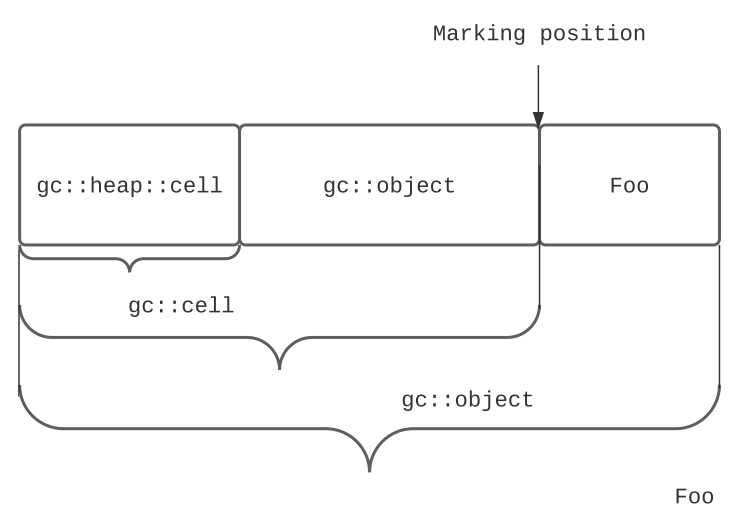
\includegraphics[scale=0.5]{./report_srcs/c_plus_plus_casting.png}
    \end{center}
\end{figure}

Because of this and the fact that a class wil inherit from the \texttt{gc::object} class, the marker is positioned to start
at \texttt{(((char*)this) + sizeof(gc::object))}

Because fields start at the beginning of the user specified section of the object, this position can be assured to start
at the initial field (if there are any)

Due to the lack of reflection, the marker needs to work out when to stop marking by analysing the data at the current marking position.
This is done based on knowledge of how a field should be formatted.

Fields have to hold a reference to an object in the heap or a nullptr in order to be valid. Both formats are easy to test:
\begin{itemize}
\item If the marker sees a nullptr at its current position it will accept this as a vliad field and move onto the next one.
\item If the marker sees a pointer address which is within the range of the heap it will mark the referemced object and then move onto
\end{itemize}
the next field.

Fields are ended with the \texttt{END\_GC\_FIELDS} macro. This macro actually adds a new member to the class of type \texttt{void*} pointing
to one position less than the allocated heap. The marker will look specifically for this pointer value when looping through 
the fields to mark. If it sees this value, it will know that it has marked the last field and can stop.
\subsubsection{Optimization Attempts for Stopping Marking}
\label{sec:orge933d6c}
A few ideas of how to stop marking were considered prior to this one in an attempt to lower the memory overhead.
The magic pointer technique requires an 8 byte overhead on 64 bit systems.

This compares to a field flag technique which would have added a byte to the top of the field class which could have a different
value to a \texttt{END\_GC\_FIELDS} added member byte at the end of the field list. This approach is better as long as a class
has fewer than 7 fields (each field has an extra byte along with the =END\textsubscript{GC}\textsubscript{FIELD} byte makes the 8 bytes taken by the pointer technique).
A slightly different approach that could be taken is to reserve the top bit of the fields pointer for use in the marking system
(set to 0 on fields),. This approach would allow for an overhead of only a single byte at the expence of reducing the addressable heap 
memory from 64 to 63 bits.

Unfortunetly due to the prominence of little endian formatted computers, applying the current system while only observing the most
significant byte cannot be used as an optimisation. On big endian machines, a magic number could be used checking only the most significant
byte and ommitting the rest of the pointer bringing the overhead back to just a single byte without reducing addressable space.
\subsection{Allocating}
\label{sec:org5874d80}
AGC oibjects have an overidden \texttt{new} operator which calls the \texttt{gc::heap::heap\_struct::malloc} function to provide a suitable memory position
in the heap.
\subsubsection{\texttt{gc::heap::heap\_struct::malloc}}
\label{sec:org761231a}

The \texttt{malloc} function uses the \texttt{attempt\_allocate} member function to find the memory position. If this function return a \texttt{nullptr}, this 
means that the function was unable to find a suitable memory position and the system should attempt a garbage collection before containing.

\texttt{malloc} will attempt to allocate twice after two gc cycles, before giving up and throwing a \texttt{bad\_alloc} exception.
The reason for the double collection is to ensuire that recently unreferenced objects have an opportunity to become freed when attempting
to allocate:

\begin{figure}[H]
    \begin{center}
    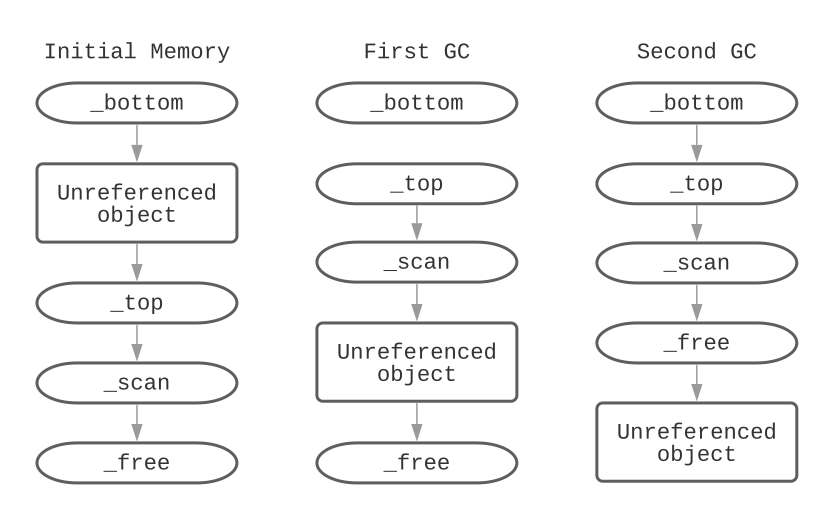
\includegraphics[scale=0.5]{./report_srcs/collecting_unreferenced_object.png}
    \end{center}
\end{figure}

If the system is unable to allocate an object after two gc rounds it is highly likely that it is not possible to allocate the given object 
(This does however depend on the number of allowed allocation loops which will be discussed with regards to the \texttt{attempt\_allocate} funcction).

Once \texttt{malloc} has been provided a suitable memory position it will re-adjust the position to take account of V-Tables.
In C++, objects that make use of virtual functions start their memory allocation with a pointer to a V-Table to perform the function lookup
AGC has two main kinds of structures that appear on the treadmill lists.
Initially the treadmill is set up with a single \texttt{gc::cell} in the free list which is the same size as the given heap size.
\texttt{gc::cell} does not have any virtual functions, and as such, does not begin its memroy allocation with a V-Table reference.
gc::object however, does start with a V-Table pointer (This is not necessarily a requirement for it to function, but is currently kept like 
this to ensure users can use virtual functions further down the inheritance tree). The \texttt{gc::object} class also inherits from the \texttt{gc::cell}
class which is the reason for the need to reposition the memory position after allocation.

Links in the treadmill list always point to the \texttt{gc::heap::cell} object. This is fine initially as the cell begins at the given pointer position:

\begin{figure}[H]
    %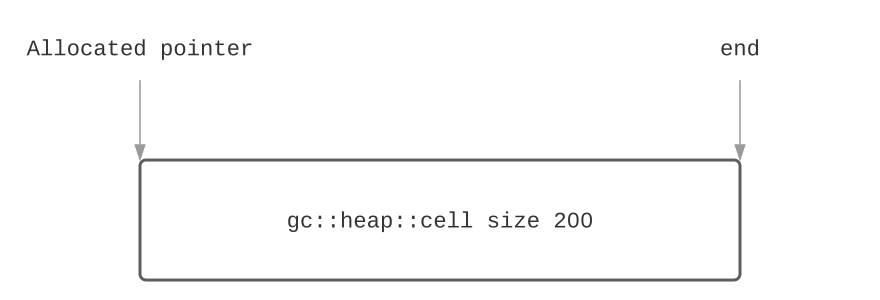
\includepdf[pages=1,viewport=-1000 -400 4000 1200, clip]{report_srcs/free_cell_allocation.pdf}
    \begin{center}
    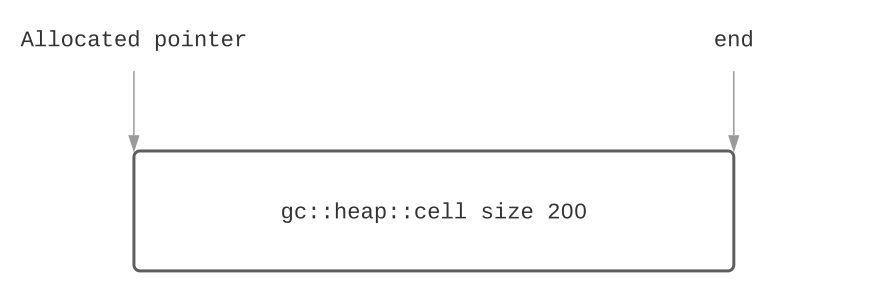
\includegraphics[scale=0.5]{./report_srcs/free_cell_allocation.png}
    \end{center}
\end{figure}

But this will not work if the cell is actually part of a now garbage collected object. In this second case the position of the cell object and
the position of where that cell actually is are different, due to the additional V-Table pointer.

\begin{figure}[H]
    %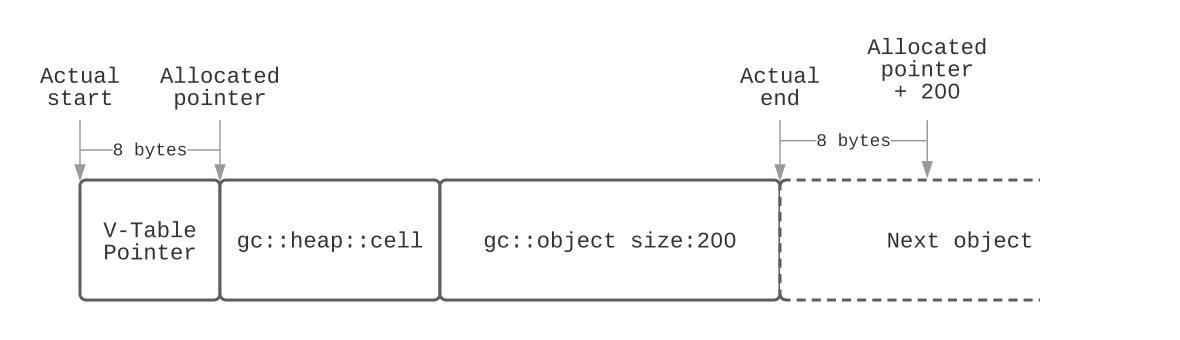
\includepdf[pages=1,viewport=-400 500 1000 1000, clip]{report_srcs/full_object_allocation.pdf}
    \begin{center}
    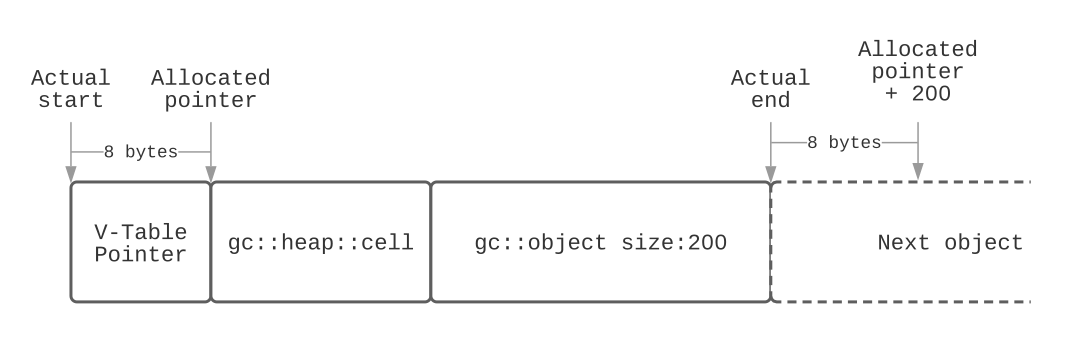
\includegraphics[scale=0.5]{./report_srcs/full_object_allocation.png}
    \end{center}
\end{figure}

\texttt{malloc} takes this information into account by calling the \texttt{gc::heap::cell::actual\_position()} member function.
The contents of this function is set when a \texttt{gc::heap::cell} is constructed and gives the data as to whether the cell object is at an offset
or not. When a standard cell is created, this function will return the same as the \texttt{this}[tr, but if it was constructed during the creation of a
gc::object it will instead point to \texttt{this - sizeof(void*)}.

\texttt{malloc} must make this adjustment to ensure that any newly created object does not bleed data into the next heap position.

\texttt{malloc} will also add this cell to the initialization list. This is a blacklist that ensures that objects do not 
get garbage collected before their initialization has been finished. Without this safety, a sub object \texttt{malloc} could run out 
memory and attempt to garbage collect its parent object's memory.
Once the entire object has been fully constructed (an event the system knows has taken place once the field/static\textsubscript{ptr} constructors have been reached),
the objects get removed from the initialization list ready for possible garbage collection.
\subsubsection{\texttt{gc::heap::heap\_struct::attempt\_allocate}}
\label{sec:org8e7a864}
This function is responsible principally for finding free memory locations, and where necessary, merging contiguous cells that exist in free memory.
\texttt{attempt\_allocate} attempts to find allocation positions by comparing the new object's size requirements to each cell in the free list, starting
from the top of the list (\texttt{\_free} cell) and working down.
If a free cell is found which is large enough, it will break off an amount of memory which is equal to the size of the new cell.

If the new object size is the same as the free cell size, this is a very simple process. All that needs to be done is to unlink the 
free cell from the free list and return the pointer.
If however the free cell is larger, a cell resize needs to take place by calling the \texttt{gc::heap::cell::resize} function.

Cell resizing is performed by moving the start of the free cell object forwards by an amount which is equal to the size of the new object.

\begin{figure}[H]
    %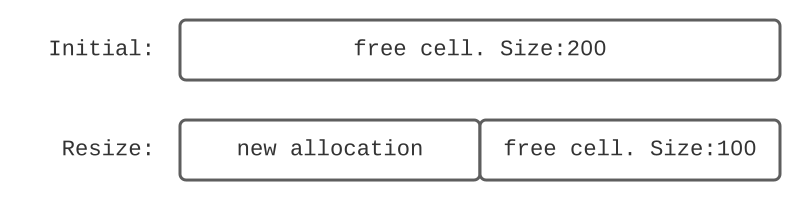
\includepdf[pages=1,viewport=-400 500 1000 1000, clip]{report_srcs/initial_to_resize.pdf}
    \begin{center}
    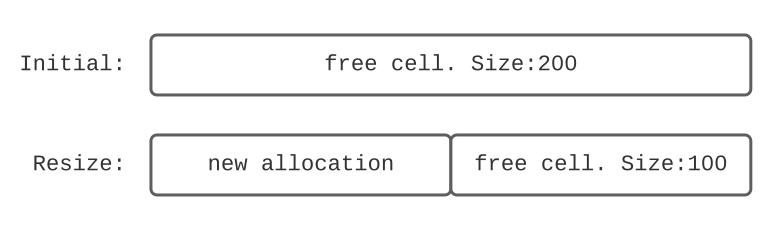
\includegraphics[scale=0.5]{./report_srcs/initial_to_resize.png}
    \end{center}
\end{figure}


\texttt{gc::heap::cell} has a certain amount of data that needs to be stored, such as its size and positions in the 
treadmill and location lists. Because of this, there is a minimum object size for a given cell. If it is found that the space left
over in the free cell is too small, a cell merge needs to be performed with one of its neighbours. \texttt{resize} will first attempt to merge
the memory with its forward neighbout if this is not allocated memory. In this case a new cell is created at the position of the 
orphan memory which will incorporate the orphan memory along with the forward cell that it is being merged with:

\begin{figure}[H]
    %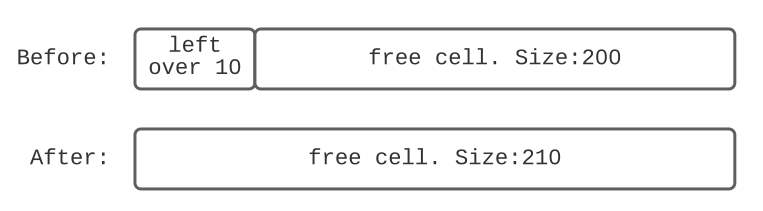
\includepdf[pages=1,viewport=-400 500 1000 1000, clip]{report_srcs/forward_merge.pdf}
    \begin{center}
    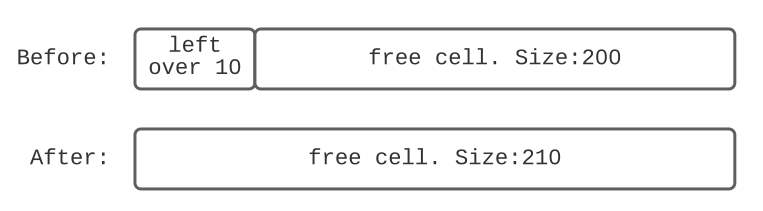
\includegraphics[scale=0.5]{./report_srcs/forward_merge.png}
    \end{center}
\end{figure}


If the forward object is allocated memory then it is noot possible to merge without corruption of the object. So instead, a merge with
the back object (or more specifically our newly allocated object) is performed which will simply act as padding on the end of the
object allocation

\begin{figure}[H]
    %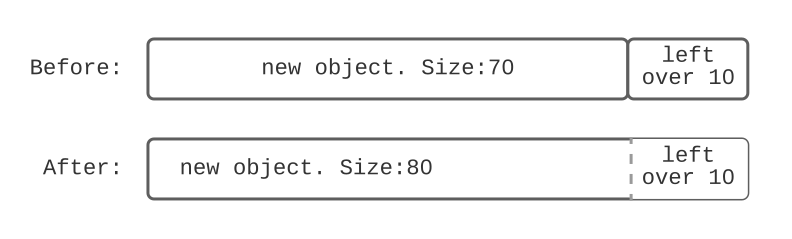
\includepdf[pages=1,viewport=-400 500 1000 1000, clip]{report_srcs/backward_merge.pdf}
    \begin{center}
    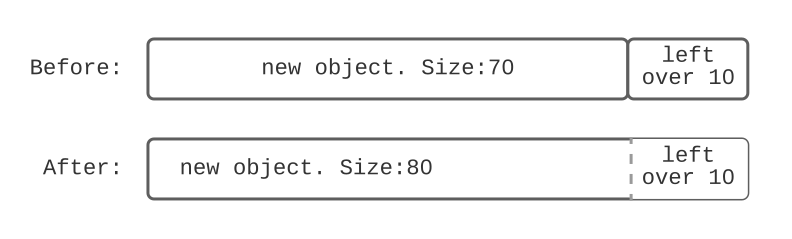
\includegraphics[scale=0.5]{./report_srcs/backward_merge.png}
    \end{center}
\end{figure}


If a free cell is not large enough to accomodate a new object size, \texttt{attempt\_allocate} will attempt to merge the current
free cell with its forward neighbour and try again. If it is unable to merge with its forward neighbout it will move onto the
next position in the free list and attempt the same algorithm again. \texttt{attempt\_allocate} has a loop limit 
defined when the heap is first created as the \texttt{gc::heap::heap\_struct::\_max\_allocation\_attempts\_before\_gc} member.
Once the \texttt{attempt\_allocate} loop has been run this many times the function will giv e up and return a nullptr in order to allow a
garbage collection to take place to free up more memory.
\subsubsection{Detecting Free Cells in O(1) Time}
\label{sec:orgf17289b}
Detecting whether or not a cell is currently free or not is important in this system to ensure that data does not get corrupted by cell
merges. Because making this check needs to be performed on such a consistent basis, it is also important that the detection
of free cells is a very fast process, in this case, an O(1) time process.

AGC's cell merge system uses the \texttt{gc::heap::cell::garunteed\_free} function to check to ensure that a cell is definetly in the free
list. It is important to note that not every free cell will return true to this function depending on its current
state. It only garuntees that no cell that returnes true to this function can not be free.

To do this, every \texttt{gc::heap::cell} has a byte member called \texttt{\_iteration}.
This value corresponds to the byte member \texttt{gc::heap::heap\_struct::\_gc\_iteration}. This number gets iterated every time a garbage collection
flip is performed and is used as a notification to all objects that their gc status has been changed.
\begin{enumerate}
\item Use on Objects That Are Still Allocated
\label{sec:org8d208fb}
Objects need to keep track of what gc list they are currently in, in a fashion which can be accessed in O(1) time. Objects
do this by using the byte member \texttt{gc::object::\_mark} which can either be \texttt{W}, \texttt{G} or \texttt{B} for \emph{ecru}, \emph{top} and \emph{bottom} lists respectively
at different makrs, the object will perform different actions when the \texttt{gc::cell::gc\_mark()} member function is called.
\begin{itemize}
\item When in \emph{ecru}, the object moves to \emph{grey} and changed \texttt{\_mark} to \texttt{G}
\item When in \emph{grey}, the object moves to \emph{black}, calls \texttt{gc::cell::gc\_mark} on all of its fields, and changes \texttt{\_mark} to \texttt{B}.
\item When in \emph{black}, no action is taken.
\end{itemize}

The \texttt{\_iteration} member becomes important once a gc flip occurs. In this case it will move object in the \emph{black} list to
the \emph{ecru} list, but the objects still display an internal \texttt{\_mark} of \texttt{B} suggesting that it thinks it is
in the bottom list and should therefore do nothing when \texttt{gc\_mark} is called.
Rather than slow down the gc flip by manually setting each object back to \texttt{\_mark = 'W'}, instead the process gets delayed by 
checking for inconsistencies between \texttt{gc::heap::cell::\_iteration} and \texttt{gc::heap::heap\_struct::\_gc\_iteration}, If when
gc\textsubscript{mark} is called, the object sees that its \texttt{\_iteration} value is behind \texttt{\_gc\_iteration}, it now knows that a gc flip has occurred since
and it needs to reset to \texttt{\_mark =} 'W'=.
\item \texttt{\_iteration} in free cell merges
\label{sec:org1ecec9e}
This same \texttt{\_iteration member is also used in determining if a cell can be merged with. Because cells that are currently allocated
are required to update their =\_iteration} member every gc cycle to keep in sink with the global \texttt{\_gc\_iteration},
this fact can then be exploited in order to tell which cells are not being updated.
It can be garunteed that any cell which has an \texttt{\_iteration} value that is not equal to \texttt{\_gc\_iteration} or
\texttt{\_gc\_iteration - 1} is actually a free cell.
\begin{itemize}
\item \texttt{\_iteration = \_gc\_iteration} must have either recently updated their member or have been allocated in the current iteration and are
\end{itemize}
therefore not free
\begin{itemize}
\item Cells that have \texttt{\_iteration = (\_gc\_iteration - 1)} must either not yet have had the change to update their mark yet, or have just
\end{itemize}
been freed in the previous cycle.

If any other \texttt{\_iteration} value is found, the we must conclude that the cell is out of date and garunteed to be free.
Because \texttt{\_iteration = (\_gc\_iteration - 1)} can be true on an allocated cell, this means that it only becomes possible to merge with
a free cell once two garbage collections have passed since it was first placed in the free list.
\end{enumerate}

\subsection{Object Survival and Being Unreferenced}
\label{sec:org57a7dd4}
The standard approach for memory mangement in C++ is to perform reference counting, that is, to count the number of references
that are pointing to a given object, and then, once no references are left, delete the object. AutoGarbage uses mark 
and sweep which will instead, as the program is being executed, gradually mark out and revealthe memory cells which are stil
being referenced. The underlying effect of this method of memory management is that objects
tend to stay allocated a little longer than they are actually required to be.
This means that the amount of memory used by a program at any time is going to be slightly greater than what is actually 
reqruied, simply because a gc cycle has yet to occur, or an object gets sent to the grey/black field just before it gets dereferenced.

This expanded object lifetime can mean that on occasion, a greater computational overhead is also associated with mark and sweep
as it can take a couple of cycles for an unreferenced object to finally be freed. Specifically in the AutoGarbage system,
it may even take yet another cycle to become a genuinely useful allocatable object, due to the approach taken to 
ensuring that it is safe to merge with free cells.
\end{document}
